\documentclass{article}
\usepackage[left=2cm,right=2cm,top=2cm,bottom=2cm]{geometry}
\usepackage{nicematrix}
\usepackage{array}
\usepackage{colortbl}
\usepackage{amssymb}
\usepackage{xcolor}
\usepackage{tabularx,multirow,hhline,colortbl}
\usepackage{hhline}
\usepackage{tikz}
\colorlet{myorange1}{orange!20}
\usepackage{circuitikz}
\colorlet{myorange2}{orange!40}
\usetikzlibrary{arrows}
\newcommand{\midarrow}{\tikz \draw[-triangle 90] (0,0) -- +(.1,0);}
\begin{document}
\begin{minipage}{.5\textwidth}%
\begin{flushleft}
\hspace*{-0.6cm}
Université Cadi Ayyad\\
\hspace*{-0.6cm}
Faculté Poly-disciplinaire de Safi\\
\hspace*{-0.6cm}
Département de Physique
\end{flushleft}
\end{minipage}%
\hfill
\begin{minipage}{.3\textwidth}%
\begin{flushright}
Année 2017-2018
\end{flushright}
\end{minipage}%

\begin{center}
\textbf{Série TD N°4}\\
Énergies et échanges du rayonnement thermique
\end{center}
\textbf{Exercice 1:}\\
Soit un cylindre compris entre $x=0~et~x=L$, de masse volumique $\rho$, de capacité thermique massique $c$ et de conductivité $K$. Le problème est unidimensionnel selon $(ox)$, la température étant considérée uniforme dans la section $S$ du cylindre. La surface latérale du cylindre est thermiquement isolée.\\
On notera $D=\frac{K}{\rho c}$.\\
Il n'y a pas de sources thermiques.
\begin{enumerate}
\item En appliquant le premier principe, établir l'équation de diffusion thermique pour la fonction $T(x,t)$.
\item On cherche des solutions de la forme $T(x,t)=f(x)g(t)$. Expliciter $f(x)~et~g(t)$.
\item Les extrémités du cylindre ont une température uniforme $T_{0}$.\\
A $t=0$, $T(x,0)=T_{1}sin(\frac{\pi x}{L})+T_{0}$.\\
Déterminer $T(x,t)$.
\end{enumerate}
\textbf{Exercice 2:}\\
On ne considère deux corps noirs dont l'un est à la température $T_{1}=2500~K$. Déterminer la température de l'autre corps noir sachant que la différence entre les deux longueurs d'onde correspondant aux maximums de leurs densités spectrales d'énergie vaut: $\lambda_{m2}-\lambda_{m1}=\Delta\lambda_{m}=0.5~\mu m$.\vspace{8px}
\\
\textbf{Exercice 3:}\\
Le soleil eut être considéré comme une sphere de rayon $R_{S}=700~000~Km$, à la température $T_{S}=5800~K$.\\
On assimile le soleil à un corps noir.
\begin{enumerate}
\item Quel est le domaine de longueur d'onde dans lequel le soleil émet majoritairement?
\item Calculer la puissance $\phi_{e}$ totale émise par le soleil. On donne: $\sigma=5.67.10^{-8}W.m^{-2}.K^{-4}$.
\item En déduire le flux surfacique $\varphi_{i}$ incident au niveau de l'orbite terrestre. La distance Terre-Soleil vaut $D=150~millions~de~Km$.
\item Quel est le flux $\phi_{i}$ total incident arrivant sur la Terre? Le rayon terrestre est $R_{T}=6~400$.
\item On suppose que la Terre est également un corps noir. Quel le flux $\phi_{a}$ absorbée par la Terre?
\item Quel est le flux $\phi^{'}_{e}$ émis par la Terre? On appellera $T_{t}$ la température de la Terre, supposée uniforme.
\item Exprimer et calculer la température de la Terre en supposant le régime stationnaire.
\end{enumerate}
\textbf{Exercice 4:}\\
Un corps sphérique (A) de rayon R, de capacité thermique $C_{0}$, et de température $T_{1}$, et placé dans une enceinte vide dont les parois intérieure absorbante est maintenue à la température $T_{0}$. On suppose que le corps (A) rayonne comme un corps noir et qu'il n'y a pas d'autres types de transferts thermiques.\\
\begin{minipage}{.65\textwidth}%
\vspace*{0.4cm}
Les températures $T_{1}$ et $T_{2}$ sont voisines et l'on pose $T_{1}=\theta + T_{0}$ avec $\theta \ll T_{0}$.
\begin{enumerate}
\item Quel est le flux $\phi_{a}$ reçu par le corps (A) de la part de l'enceinte.
\item Déterminer la loi d'évolution de la température T de la sphère en fonction du temps.
\item On considère une sphère métallique de rayon R=1cm, de capacité thermique massique $c=0.5kJ.K^{-1}.Kg^{-1}$.\\
Données: $T_{0}=273K$, $T_{1}=280K$ et la constante de Stefan: \\ $\sigma=5.67.10^{-8}W.m^{-2}.K^{-4}$.
\end{enumerate}
\end{minipage}%
\hfill
\hspace*{1.75cm}
\begin{minipage}{.35\textwidth}%
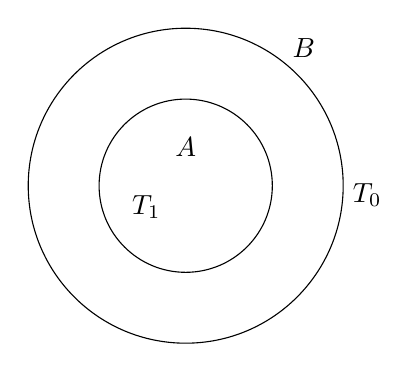
\begin{tikzpicture}
\draw (-0.5,0) node[below]{$T_{1}$} ;
\draw (0,0.25) node[above]{$A$} ;
\draw (2,-0.12) node[right]{$T_{0}$} ;
\draw (1.5,1.5) node[above]{$B$} ;
\draw (0,0) circle (1.1) ;
\draw (0,0) circle (2) ;
\end{tikzpicture}
\end{minipage}%
\vspace*{0.4cm}
Au bout de combien de temps, l'écart de température $(T-T_{0})$ est-il inférieur à 0.1 K?
\\
\textbf{Exercice 5:}\\
La Terre est assimilée à un corps noir de température $T_{t}$, émettant un rayonnement thermique de flux surfacique $\varphi_{t}$. La Terre est supposée entourée d'une couche contenant du dioxyde de carbone gazeux en concentration $C_{0}$ fixée. La température de cette couche est notée $T_{c}$ et le rayonnement qu'elle émet est associée au flux surfacique $\varphi_{c}$ des deux c\^otés  de la couche.\\
On désigne par $\varphi_{s}$ le lux solaire surfacique reçu. Les rayons solaires arrivent sous incidence normale sur la couche gazeuse.
\begin{enumerate}
\item \begin{enumerate}
\item[a.] Rappeler la forme de la loi du déplacement de Wien.
\item[b.] On sait que le Soleil, de température $T_{S}=6000K$, émet un rayonnement situe dans le domaine visible $\lambda_{m}=0.5\mu m$. En utilisant un ordre de grandeur raisonnable pour les températures, déterminer approximativement la longueur d'onde d'émission radiative maximale de la Terre et de la couche de $CO_{2}$.
\end{enumerate}
\item On admettra par la suite que l'absorption de $\varphi_{t}$ par la couche de $CO_{2}$ est totale et que cette couche peut donc être assimilée à un corps noir dans le domaine spectral du flux radiatif terrestre, mais elle est transparente au rayonnement solaire ($\varphi_{S}$ le flux solaire surfacique).
\item[a.] Traduire l'équilibre radiatif de l'ensemble {couche gazeuse + Terre}; on supposera que la Terre et la couche gazeuse ont sensiblement le même rayon, et donc la même surface émissive d'un coté.\\
Traduire l'équilibre de la Terre seule.
\item[b.] Exprimer la température $T_{t}$ en fonction de $\varphi_{S}$ et de la constante de Stefan. Comparer le résultat à celui que l'on obtiendrait si la couche n'existait pas.\\
Application numérique:
\begin{center}
$\varphi_{S}=342~W.m^{-2}$\\
$\sigma=5.67.10^{-8}W.m^{-2}.K^{-4}$
\end{center}
\item On suppose que la quantité $CO_{2}$ augmente. On modélise cette augmentation en considérant la superposition de $N$ couches contenant du $CO_{2}$, toutes identiques à la précédente. Ainsi, chaque couche admet la même concentration en $CO_{2}$. On note $\varphi_{cp}$ le rayonnement émis vers le haut et vers le bas par la $P^{ieme}$ couche de température $T_{cp}$. Le rayonnement émis par une couche est totalement absorbe par les autres couches.
\item[a.] Traduire l'équilibre radiatif en terme de flux surfacique:
\begin{enumerate}
\item[$\bullet$] L'ensemble {toutes les couches + Terre};
\item[$\bullet$] La couche p;
\item[$\bullet$] La première couche;
\item[$\bullet$] La Terre.
\end{enumerate}
\item[b.] En déduire $\varphi_{cp}$ et $\varphi_{t}$ en fonction de $\varphi_{S}$, de $N$ et de $\sigma$.
\item[c.] Donner finalement l'expression de $T_{t}$ en fonction de $\varphi_{S}$, de $N$ et de $\sigma$. Conclure sur l'influence de $N$ sur $T_{t}$.
\end{enumerate}
\textbf{Exercice 6:}\\
Soit $S_{1}$ une surface convexe complètement entourée par une surface $S_{2}$. On suppose que les températures $T_{1}$ et $T_{2}$ ainsi que les émissivités $\varepsilon_{1}$ et $\varepsilon_{2}$ des deux surfaces sont connues.
\begin{enumerate}
\item Déterminer le flux net perdu par chacune de ces surfaces en utilisant le schéma électrique équivalent.
\item On suppose que la surface $S_{1}$ et petite devant la surface $S_{2}$. Simplifier l'expression du flux perdu par chacune des surfaces. Conclure.
\end{enumerate}
\textbf{Exercice 7:}\\
Un radiateur infrarouge, constitue d'une plaque chauffante carrée de c\^oté  $a=20~cm$, est placée horizontalement à une hauteur $h=4~m$ du sol.\\
\begin{enumerate}
\item La température du radiateur est égale à $T=900K$. Calculer la puissance P dissipée par le radiateur. ($\sigma=5.67.10^{-8}W.m^{-2}.K^{-4}$).
\end{enumerate}
\begin{minipage}{.65\textwidth}%
\vspace*{0.4cm}
\begin{enumerate}
\item[2.] On admet qu'une surface $dS$ d'un écran situé dans la direction i, normalement au rayonnement émis par le radiateur et à une distance r du radiateur, reçoit une puissance:\\
$dP=La^{2}\cos i \frac{dS}{r^{2}}$\\
Où L est la luminance énergétique.\\
Déterminer L en fonction de $\sigma$ et $T$.
\end{enumerate}
\end{minipage}%
\hfill
\hspace*{1.75cm}
\begin{minipage}{.35\textwidth}%
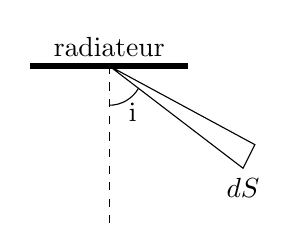
\begin{tikzpicture}
\draw[line width=2pt] (-1,0) -- (1,0) ;
\draw[dashed] (0,0) -- (0,-2) ;
\draw (0,0) -- (1.85,-1) -- (1.7,-1.3) --  cycle;
\draw (0,-0.5) arc (270:330:0.43);
\draw (0,0) node[above]{radiateur} ;
\draw (0.3,-0.35) node[below]{i} ;
\draw (1.7,-1.3) node[below] {$dS$} ;
\end{tikzpicture}
\end{minipage}%
\\
\begin{minipage}{.65\textwidth}%
\vspace*{0.4cm}
\begin{enumerate}
\item[3.] En déduire le flux surfacique pour un point du sol situé:
\begin{enumerate}
\item[a.]en A, à la verticale du radiateur;
\item[b.]en B, à une distance d=3cm de A.
\end{enumerate}
\end{enumerate}
\end{minipage}%
\hfill
\hspace*{1.58cm}
\begin{minipage}{.35\textwidth}%
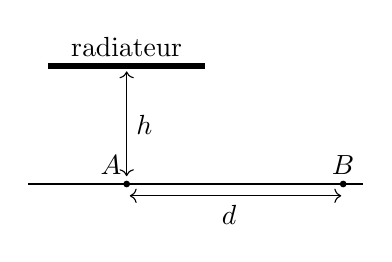
\begin{tikzpicture}
\draw[line width=2pt] (-1,0) -- (1,0) ;
\draw[<->] (0,-0.07) -- (0,-1.4) ;
\draw (-1.25,-1.5) -- (3,-1.5) ;
\draw[<->] (0.04,-1.65) -- (2.725,-1.65) ;
\draw (0,0) node[above]{radiateur} ;
\draw (0,-0.75) node[right]{$h$} ;
\draw (2.75,-1.5) node[above]{$B$} ;
\draw (-0.2,-1.5) node[above]{$A$} ;
\draw (1.3,-1.65) node[below]{$d$} ;
\draw[fill] (2.75,-1.5) circle [radius=1pt];
\draw[fill] (0,-1.5) circle [radius=1pt];
\end{tikzpicture}
\end{minipage}%
\\
\textbf{Exercice 8:}\\
Une petite bille sphérique de cuivre, assimilée à un corps noir, de diamètre $D=30mm$, de chaleur massique $c=390J.K^{-1}.Kg^{-1}$ et de masse volumique $\rho=8.9~10^{3}~Kg.m^{-3}$, est à la température $T_{0}=288K$ à l'instant $t=0$.\\
On place cette bille dans un enceinte vide dont la paroi intérieure est maintenue à température constante $T_{1}=300K$; On donne $\sigma=5.67.10^{-8}W.m^{-2}.K^{-4}$.
\begin{enumerate}
\item Établir l'équation différentielle qui régit l'évolution de la température $T()t$ de la sphère au cours du temps.
\item En tenant compte des faibles écarts de température $(T(t)-T_{1}\ll T_{1})$, établir la loi de (t); calculer la constante de temps $\tau$ de cette évolution.
\item Calculer, à l'instant $t=\tau$, le flux radiatif à la surface de la bille et la vitesse d'échauffement $\frac{dT}{dt}$.
\item Déterminer à quel instant la bille atteint la température moyenne $T_{m}=\frac{T_{0}+T_{1}}{2}$.
\end{enumerate}
\end{document}